\documentclass{article}
\usepackage[english,russian]{babel}
\usepackage[utf8]{inputenc}
\usepackage{indentfirst}
\usepackage{graphicx}
\usepackage{float}
\usepackage[margin=2cm]{geometry}

\begin{document}
\begin{titlepage}
	\begin{center}
    	ГУАП
    	\vspace{0.25cm}

    	КАФЕДРА №51
	\end{center}

    \begin{flushleft}

    	ОТЧЕТ

    	ЗАЩИЩЕН С ОЦЕНКОЙ

		ПРЕПОДАВАТЕЛЬ


    	\vspace{0.5cm}

		$\rule{5cm}{0.15mm}$ \hfill $\rule{2.2cm}{0.15mm}$  \hfill $\rule{3.25cm}{0.15mm}$

		должность, уч. степень, звание \hfill подпись, дата \hfill инициалы, фамилия
    \end{flushleft}

 	
    \hspace{2cm}

	\begin{center}
    	ОТЧЕТ ПО ЛАБОРАТОРНОЙ РАБОТЕ №8


    	\vspace{1cm}

    	THREAD


    	\vspace{1cm}

    	по курсу: ОСНОВЫ ПРОГРАММИРОВАНИЯ {\MakeUppercase{\romannumeral 2}}
    \end{center}

    \vspace{3cm}

    \begin{flushleft}
    	РАБОТУ ВЫПОЛНИЛ

    	СТУДЕНТ ГР. № 5511 \hfill $\rule{2.2cm}{0.15mm}$  \hfill $\rule{3.25cm}{0.15mm}$

    	\hspace{7.8cm} подпись, дата \hfill инициалы, фамилия
    \end{flushleft}

	\vspace{5cm}
	\begin{center}
 		Санкт-Петербург, 2017
	\end{center}
\end{titlepage}

\section{Задание}
Реализовать класс ThreadedMatrixProduct для многопоточного умножения матриц UsualMatrix. В конструкторе класс получает число потоков, которые будут использованы для перемножения (число потоков может быть меньше, чем число строк у первой матрицы).

В функции main сравнить время перемножения больших случайных матриц обычным и многопоточным способом. Получить текущее время можно с помощью методов класса System.


\section{Дополнительное задание}
Реализовать многопоточное переборное решение задачи о рюкзаке.

\section{Реализация}
\subsection{Основное задание}
Для многопоточного перемножения матриц созданы отдельные классы ThreadedMatrixProduct и MultiplicationThread.\\

Класс MultiplicationThread наследован от класса Thread, хранит значения результирующей и перемножаемых матриц, номера строк в диапазоне которых будет происходить умножение.  В переопределенном методе run() происходит перемножение выделенной части матрицы.\\

У класс ThreadedMatrixProduct есть метод threadedProduct, который получает в качестве параметров первую и вторую матрицы, а так же количество потоков, с помощью которых будет перемножаться матрица.
Данный метод расчитывает количество элементов матрицы, которые должен расчитать каждый поток. Затем в цикле создаются MultiplicationThread, которым в конструкторе передаются необходимые параметры, а именно матрицы для перемножения, результирующая матрица, а так же начальный и конечные индексы в матрице для вычисления.  

\subsection{Дополнительное задание}
Для многопоточного решения задачи о рюкзаке методом перебора были созданы классы Knapsack и Item. \\
Класс Item, хранит информацию о предмете, а именно имя, стоимость и вес.

У класса Knapsack существует два главных публичных метода:
\begin{itemize}
	\item findBestCombination(ArrayList<Item> items), ищущий лучшую комбинацию из доступного списка предметов, рекурсивным методом. 
	\item threadedFindBestCombination(ArrayList<Item> items, int threadCount), который ищет лучшую комбинацию, разбивая доступный список по потокам и вызывая не многопоточный поиск лучшей комбинации для каждого потока. 
\end{itemize}

\section{Инструкция}
При запуске программы основного задания она последовательно выводит на экран:
\begin{itemize}
	\item Время и результат перемножения матриц на 42 потоках.

	\item Время и результат перемножения матриц на 4 потоках.
\end{itemize}

При запуске программы дополнительного задания она последовательно выводит на экран:
\begin{itemize}
	\item Время и результат решения задачи о рюкзаке с заданными параметрами рекурсивным методом.

	\item Время и результат решения задачи о рюкзаке с заданными параметрами многопоточным методом.
\end{itemize}

\section{Тестирование}

\subsection{Пример запуска программы}
\begin{figure}[H]
	\begin{flushleft}
		\centerline{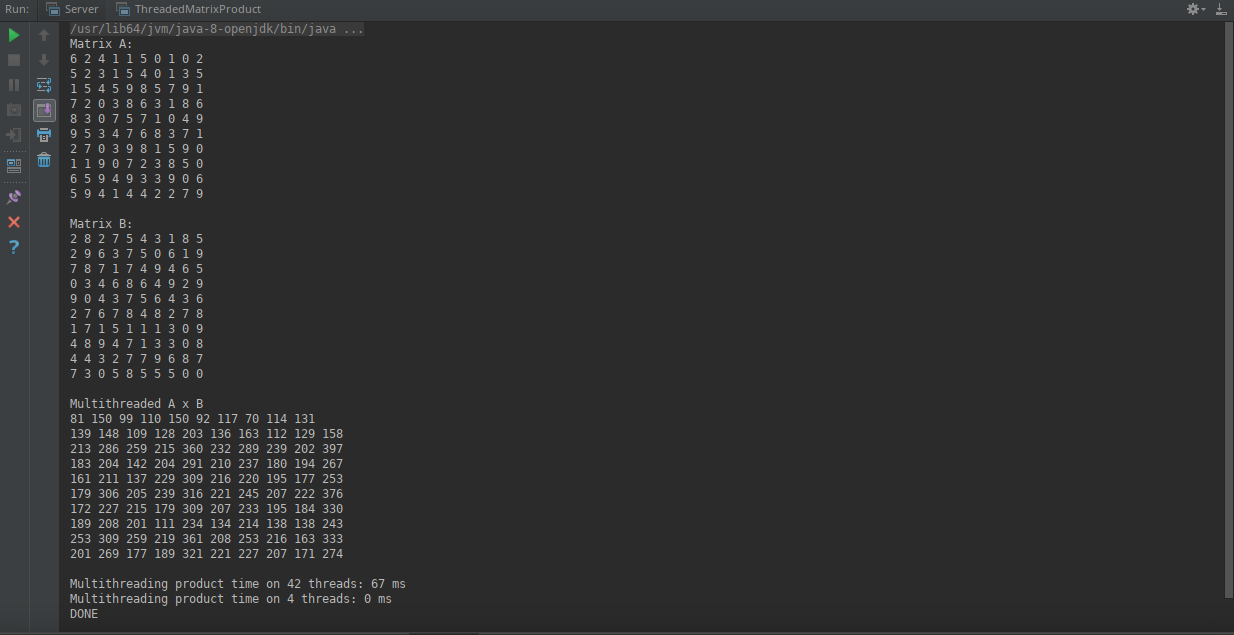
\includegraphics[scale=0.55]{lab8_main.png}}
		\caption{Пример работы программы основного задания}
	\end{flushleft}
\end{figure}
\begin{figure}[H]
	\begin{flushleft}
		\centerline{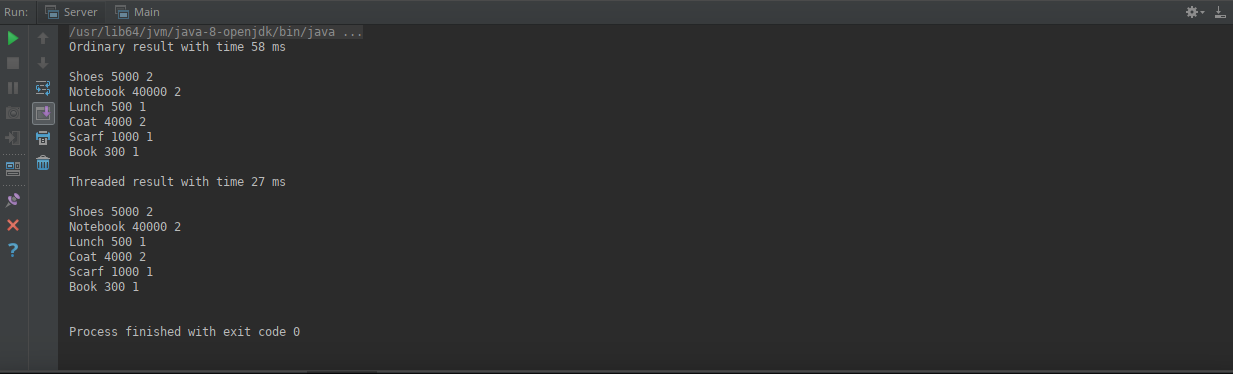
\includegraphics[scale=0.55]{lab8_add.png}}
		\caption{Пример работы программы дополнительного задания}
	\end{flushleft}
\end{figure}

\end{document}
